\documentclass[conference]{IEEEtran}
\IEEEoverridecommandlockouts
% The preceding line is only needed to identify funding in the first footnote. If that is unneeded, please comment it out.
\usepackage{cite}
\usepackage{amsmath,amssymb,amsfonts}
\usepackage{algorithmic}
\usepackage{graphicx}
\usepackage{textcomp}
\usepackage{xcolor}
\usepackage{url}
\usepackage{float}
\usepackage[T1]{fontenc}
\usepackage[utf8]{inputenc}
\def\BibTeX{{\rm B\kern-.05em{\sc i\kern-.025em b}\kern-.08em
    T\kern-.1667em\lower.7ex\hbox{E}\kern-.125emX}}
\begin{document}

\title{Zvučni efekti na gitari\\
%{\footnotesize \textsuperscript{*}Note: Sub-titles are not captured in Xplore and
%should not be used}
%\thanks{Identify applicable funding agency here. If none, delete this.}
}

\author{\IEEEauthorblockN{Magdalena Halusek}
\IEEEauthorblockA{\textit{dept. name of organization (of Aff.)} \\
\textit{name of organization (of Aff.)}\\
City, Country \\
email address}\\
\IEEEauthorblockN{Ivana Šarić}
\IEEEauthorblockA{\textit{dept. name of organization (of Aff.)} \\
\textit{name of organization (of Aff.)}\\
City, Country \\
email address}
\and
\IEEEauthorblockN{Katarina Prgeša}
\IEEEauthorblockA{\textit{dept. name of organization (of Aff.)} \\
\textit{name of organization (of Aff.)}\\
City, Country \\
email address}\\
\IEEEauthorblockN{Ivana Žeger}
\IEEEauthorblockA{\textit{dept. name of organization (of Aff.)} \\
\textit{name of organization (of Aff.)}\\
City, Country \\
email address}
\and
\IEEEauthorblockN{Karla Salamun}
\IEEEauthorblockA{\textit{dept. name of organization (of Aff.)} \\
\textit{name of organization (of Aff.)}\\
City, Country \\
email address}
}

\maketitle

\renewcommand{\figurename}{Slika}

\begin{abstract}
sažetak??
\end{abstract}

\section{Uvod}
Zvuk je mehanički val koji se prenosi određenim medijem. Ljudsko uho je osjetljivo na
frekvencije između otprilike 20 Hz i 20 000 Hz. Jedan je od mnogih oblika kontinuiranih;
analognih signala naše okoline. Ljudski interes za fenomen zvuka traje od najranije povijesti. Do
današnjice je razvijena čitava kultura i tehnologija koja omogućuje stvaranje, snimanje, obradbu
i prijenos zvuka. Pojam koji obuhvaća i isprepliće znanost i umjetnost, a koji je povezan sa zvukom
je glazba. S ciljem što boljeg doživljaja glazbe, audio signali se obrađuju u kontinuiranoj i
diskretnoj domeni. Mikrofon pretvara zvučne valove u analogni električni sinusni signal. Taj je
signal određen jedinstvenom frekvencijom, brzinom, odstupanjima, itd. Obradba analognim
sklopovima podložna je pogreškama uzrokovanih šumom, preslušavanjem vodova,
temperaturnom ovisnošću, netočnostima nominalnih iznosa elemenata, itd. Da bi se kvalitetno
obradio, kontinuirani signal je potrebno digitalizirati. Digitalna obrada signala se provodi u
računalima. Ima brojne prednosti, poput neosjetljivosti na šum i starenje, laku prilagodbu na
nove zadatke, programabilnost.

Tema projekta je konstruiranje filtara za dodavanje efekata, digitalna obradba snimljenog zvuka
gitare primjenom istih te ispitivanje njihovog utjecaja na signal u vremenskoj i frekvencijskoj
domeni. Razvoj instrumenata i postupaka digitalne obradbe omogućio je eksperimentiranje
zvukom. Glazba se često razvijala upravo iz razloga što su pojedine slučajne greške u sviranju
instrumenata i obradbi snimaka zvuka postale utjecajni zvučni efekti. Zvučni efekti su pojam koji
obuhvaća hardver i softver odgovoran za manipulaciju zvukom. Moguće ih je dodati zvuku u
procesu nastajanja s ciljem da kasnije budu filtrirani ili preoblikovani, ili
na kraju obrade, u produkcijskoj fazi. Ne postoji jedinstveno pravilo koje je potrebno slijediti pri
odabiru redoslijeda primjene efekata~\cite{b1}. No, promijenjeni redoslijed uzrokuje promjenu zvuka.
Potrebno je voditi računa o spomenutom obzirom na zvuk koji je poželjno stvoriti. Iako postoje
mnoge vrste i podjele, kao temeljna podjela digitalnih zvučnih efekata
može se navesti sljedeća:

\begin{itemize}
	\item{modulacijski efekti – \textit{Chorus}, \textit{Tremolo}, \textit{Flanger}, \textit{Phaser},}
	\item{vremenski efekti – \textit{Reverb}, kašnjenje, odjek,}
	\item{spektralni efekti – ekvilizacija, \textit{Panning},}
	\item{dinamički efekti – kompresija i distorzija.}
\end{itemize}

Tipični redoslijed efekata za gitaru~\cite{b1} jest kompresija – distorzija – ekvilizacija – smanjenje šuma
– modulacija – kašnjenje – odjek.

Filtri po definiciji uklanjaju ili atenuiraju određene frekvencije iz spektra signala iznad
ili ispod neke granične frekvencije. Izjednačivači, pak, pojačavaju ili smanjuju određene frekvencijske
pojaseve, dok druge ne mijenjaju.



\section{Kompresija}

Kompresor djeluje na zvučni signal u cijelosti s ciljem kontrole zvuka i stvaranja \textit{sustain}
efekta. Kompresija je, zapravo, automatska kontrola glasnoće. Zadaća kompresora je smanjenje
dinamičkog raspona signala, tj. varijacije između najglasnijih i najtiših dijelova signala.
Dijelovi signala s velikim amplitudama, odnosno oni glasniji od nekog praga su atenuirani. Oni s
najmanjim amplitudama, tj. tiši od nekog praga su pojačani s namjerom postizanja uravnoteženijeg zvuka
bez distorzije. Kompresijom je omogućeno pojačanje signala bez potrebe za rezanjem (\textit{clippingom}).
Rezultat je dotjeraniji zvuk. Ipak, javlja se potreba za oprezom jer prekomjerna kompresija stvara
zašumljen i bezizražajan zvuk. Gubitak dijela dinamike postaje zamjetan pri slušanju.\\
Našim projektom napravljen je kod za usporedbu originalnog i komprimiranog signala u vremenskoj i
frekvencijskoj domeni. Blok dijagram kompresora prikazan je slikom \ref{kompresija}.

\begin{figure}[H]
    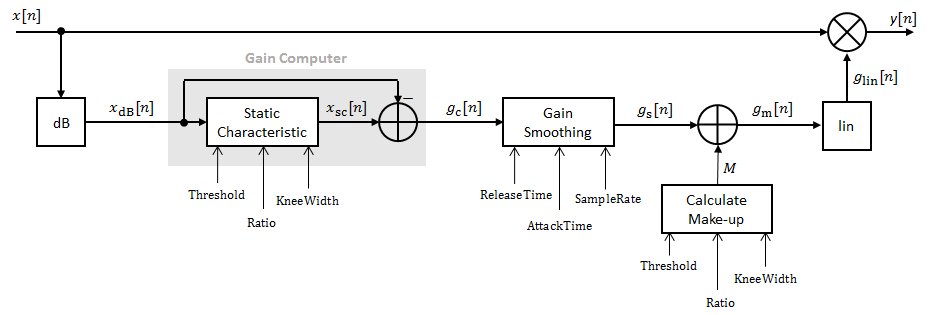
\includegraphics[width=200pt]{slike/kompresija.png}
    \centering
    \caption{Blok dijagram kompresora}
    \label{kompresija}
\end{figure}

Diskretizirani ulazni signal se pretvara u decibele radi intuitivnijih prikaza %(izbaciti ovo i početi od parametara?)
 operacija, a nakon kompresije se vraća u linearnu domenu. Glavni parametri kompresije su ~\cite{b3}:
 \begin{itemize}
   \item{prag (\textit{Treshold}) – razina ulaznog signala koja određuje početak kompresije,}
   \item{omjer kompresije (\textit{Ratio}) – omjer promjene signala na ulazu i izlazu,}
   \item{pojačanje (\textit{Make-up gain}) – pojačanje ukupne razine signala,}
   \item{vrijeme reakcije (\textit{Attack time}) – vrijeme koje je potrebno da kompresor počne djelovati na
   amplitudu signala prema definiranom omjeru kompresije nakon što signal prijeđe prag,}
   \item{vrijeme otpuštanja (\textit{Release time}) – vrijeme koje je potrebno da kompresor prestane djelovati na
   amplitudu signala i vrati se omjer kompresije 1:1 nakon što signal ponovno prijeđe prag,}
   \item{koljeno (\textit{Knee}) – prijelazno područje u izlaznoj karakteristici kompresora, %izlaznoj=prijenosnoj?
   mjesto dodira signala i linije praga.}
 \end{itemize}

 Manipulacija spomenutih parametara rezultira različitim oblicima zvuka. Promjena koljena određuje koliko će
 „glatko“ kompresor rezati signal. Promjena vremena reakcije i otpuštanja također djeluje na uglađenost zvuka.
 Što su parametri manji, to će kompresoru trebati manje vremena za početak djelovanja na amplitudu pa će signal
 zvučati dotjeranije. Najveće promjene zvuka događaju se mijenjanjem praga jer on određuje koliko će posla imati
 kompresor i koliko će „zamaskirati“ originalni signal. Za optimalne parametre prema ~\cite{b2}, dobije se vidljiva
 razlika u vremenskoj domeni, što je prikazano na slikama \ref{ulaz_vrijeme} i \ref{komp_vrijeme}.
 Primjećujemo smanjenu razliku između dijelova signala s najvišim i najnižim amplitudama.

% Ovim projektom napravljen je kod za usporedbu originalnog i komprimiranog signala u vremenskoj i
% frekvencijskoj domeni što je vidljivo na slici \ref{komp_vrijeme}.

\begin{figure}[H]
    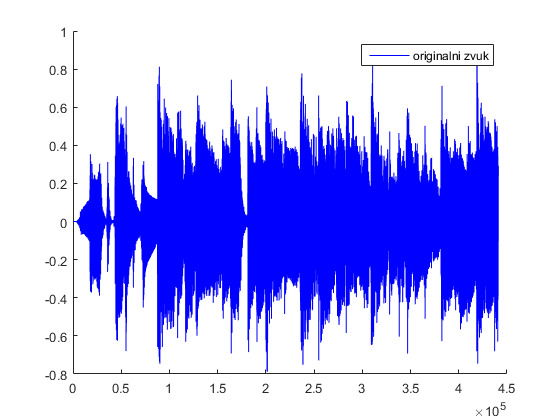
\includegraphics[width=200pt]{slike/def_orig.jpg}
    \centering
    \caption{Originalni signal u vremenskoj domeni}							%dodati legend u matlabu
    \label{ulaz_vrijeme}
\end{figure}

\begin{figure}[H]
    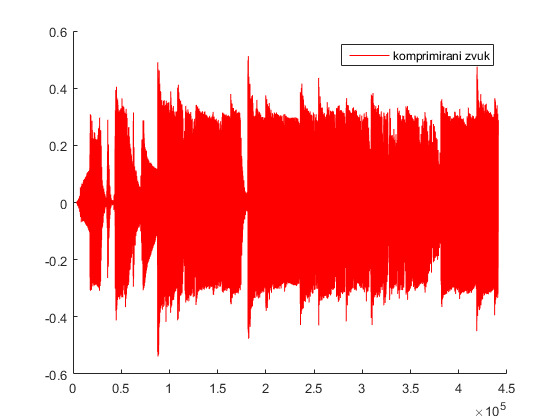
\includegraphics[width=200pt]{slike/def_kompr.jpg}
    \centering
    \caption{Komprimirani signal u vremenskoj domeni}							%dodati legend u matlabu
    \label{komp_vrijeme}
\end{figure}

% Na slici \ref{komp_spektar} vidljiva je razlika u spektru. Budući da se događaju promjene u amplitudi u
% vremenskoj domeni, to je u frekvencijskoj domeni vidljivo kao novonastala istosmjerna komponenta.
Na idućim slikama vidljiva je razlika u spektru. Budući da se događaju promjene u amplitudi u vremenskoj domeni,
to je u frekvencijskoj domeni vidljivo kao novonastala istosmjerna komponenta.

\begin{figure}[H]
    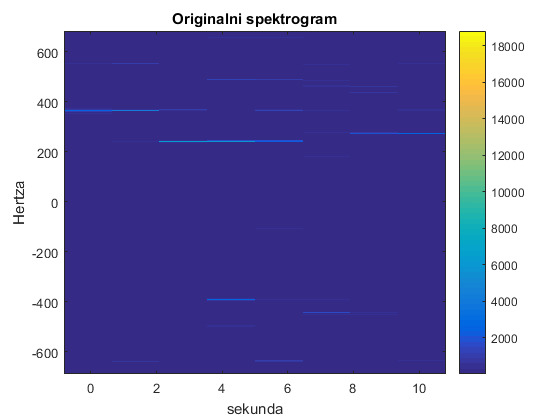
\includegraphics[width=200pt]{slike/originalni_spektrogram.jpg}
    \centering
    \caption{Spektrogram originalnog signala}
    \label{komp_ulaz_spektar}
\end{figure}

\begin{figure}[H]
    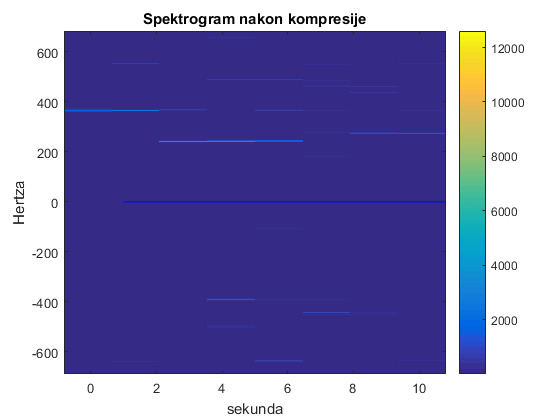
\includegraphics[width=200pt]{slike/spektrogram_nakon_kompresije.jpg}
    \centering
    \caption{Spektrogram komprimiranog signala}							%zasto DC komponenta??
    \label{komp_spektar}
\end{figure}

Kao što je već spomenuto, prekomjerna kompresija može utjecati na stvaranje zašumljenog, bezizražajnog
zvuka kao što je prikazano na slici \ref{komp_sum}. U ovom slučaju problem je prenizak prag.

\begin{figure}[H]
    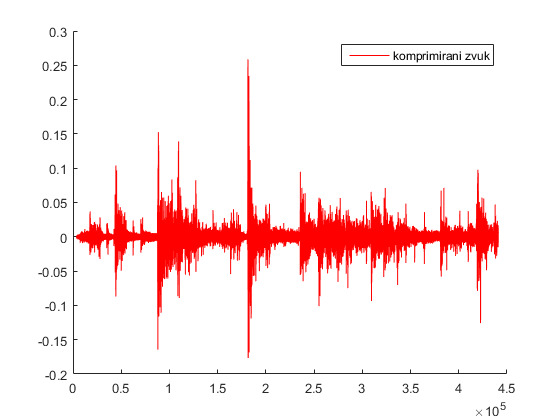
\includegraphics[width=200pt]{slike/prenizak_prag.jpg}
    \centering
    \caption{Spektrogram komprimiranog signala}
    \label{komp_sum}
\end{figure}

U spektru je šum vidljiv kao nove spektralne komponente.

\section{\textit{Flanger}}

\textit{Flanger} je zvučni efekt koji na ulazni signal unosi kašnjenje promijenjivog iznosa (najčešće manje
od 15 ms), te zakašnjeli signal dodaje na ulazni. Pritom se iznos kašnjenja mijenja kao sinusni signal
niske frekvencije - LFO (engl. \textit{Low Frequency Oscillator}, tipično 0.1 - 5 Hz)~\cite{b1}.
Primjena \textit{flanger} efekta svodi se, dakle, na dodavanje fazno moduliranog ulaznog signala na izvorni
signal. Na slici \ref{flang_simulink} prikazan je blok-dijagram FIR filtra kojim se realizira \textit{flanger}
efekt.

\begin{figure}[H]
    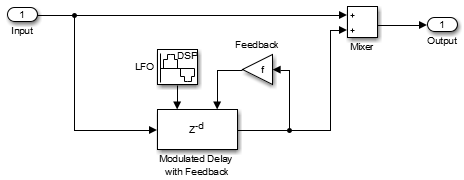
\includegraphics[width=200pt]{slike/flanger_simulink.png}
    \centering
    \caption{Blok-dijagram filtra za realizaciju \textit{flanger} efekta~\cite{b4}}
    \label{flang_simulink}
\end{figure}

FIR filtar koji se temelji na kašnjenju može se prikazati jednadžbom diferencija:
\begin{equation}
  y[n]=x[n]+g\*x[n-M]
  \label{flanger}
\end{equation}
gdje je $M$ promijenjivi iznos kašnjenja, a $g$ faktor kojim se pojačava ili atenuira zakašnjeli signal.
Budući da je iznos kašnjenja na izlazu iz LFO realan broj, prije modulacije potrebno je provesti zaokruživanje
na cijeli broj ili interpolaciju kojom se usrednjava vrijednost dvaju susjednih uzoraka.

Zvuk na koji je primijenjen \textit{flanger} prepoznatljiv je po efektu koji se popularno naziva
\textit{whooshing}. Taj se efekt javlja zbog konstruktivne i destruktivne interferencije između kombiniranih
zvučnih valova.

Slika \ref{flang_spektar} prikazuje spektrogram signala na koji je pimijenjen \textit{flanger} uz LFO
frekvenciju 1 Hz, maksimalni iznos kašnjenja 5 ms te faktor pojačanja $g=0.7$. U odnosu na spektrogram originalnog
signala koji je prikazan slikom \ref{komp_ulaz_spektar}, vidljive su nove komponente koje su nastale uslijed
modulacije zakašnjelog ulaznog signala.

\begin{figure}[H]
    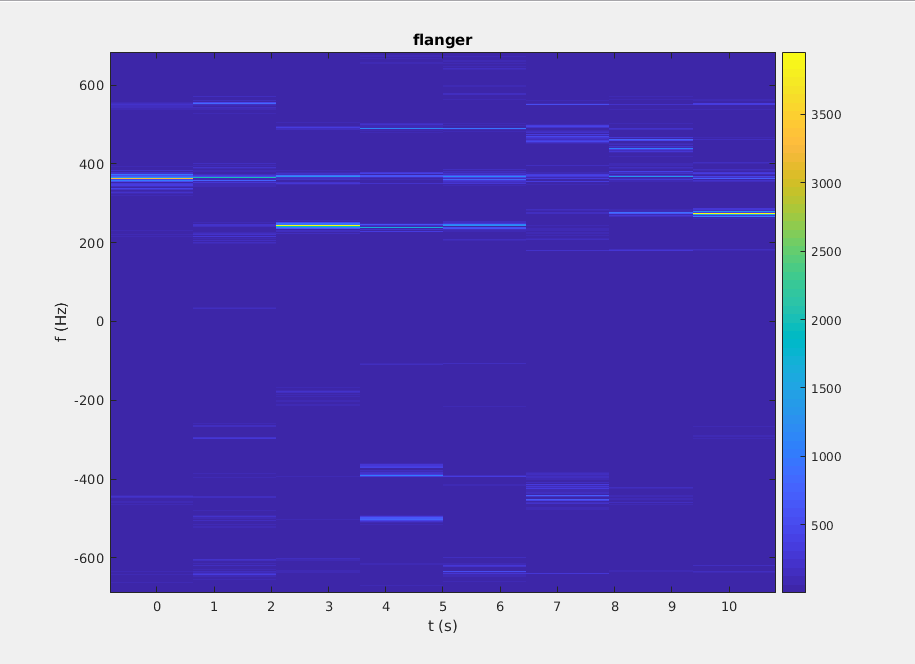
\includegraphics[width=200pt]{slike/flanger_spektar.png}
    \centering
    \caption{Spektrogram signala s \textit{flanger} efektom}
    \label{flang_spektar}
\end{figure}

\section{Odjek}

Efekt odjeka temelji se na efektu kašnjenja, koji se može opisati kao snimanje, odnosno otipkavanje, ulaznog signala
koji se zatim reproducira nakon određenog vremena. Signal kojemu je dodan efekt kašnjenja, može se
reproducirati više puta ili se ponovno snimiti što stvara ponavljajući zvuk. Osnovna struktura kašnjenja može
se ostvariti pomoću FIR ili IIR filtra ili kombinacijom dvaju filtara, gdje se efekt odjeka realizira pomoću
jednostavnog FIR filtra danog jednažbom (\ref{flanger}).
Gdje je: \[M = \tau/f_{s}\]
a $\tau$ i $f_{s}$:
 \begin{itemize}
   \item{$\tau$ - iznos kašnjenja signala,}
   \item{$f_{s}$ - frekvenciju otipkavanja.}
 \end{itemize}
Dodavanjem efekta odjeka na osnovni signal zvuk poprima dojam odbijanja zvuka od zida, dok se zapravo čuje
ponavljanje osnovnog signala. MATLAB model opisanog efekta dan je slikom \ref{echo_model}. Dodatni efekt povezan
s odjekom je efekt koji nastaje zbog povratne veze, a čuje se kao zvuk koji postepeno nestaje~\cite{b4}. Drugim riječima
vrijednost povratne veze određuje broj odjeka na način da neki postotak izlaza prosljeđuje na ulaz.
Model opisuje već danu jednadžbu FIR filtra uz dodatak povratne veze. Vrijednost $d$ u modelu odgovara vrijednosti
$M$ u jednadžbi filtra, a $f$ (\textit{FeedbackLevel}) pojačanje linije s dodanim efektom odjeka.

\begin{figure}[H]
    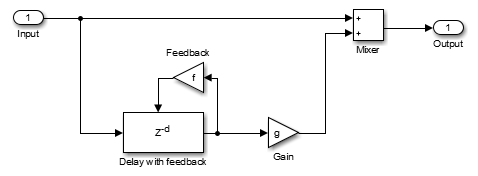
\includegraphics[width=200pt]{slike/echo_matlab.png}
    \centering
    \caption{MATLAB model odjeka}
    \label{echo_model}
\end{figure}

Na slici \ref{ulaz_vrijeme} prikazan je ulazni signal u vremenu, a na slici \ref{echo_vrijeme} prikazan je signal
u vremenu na koji je dodan efekt odjeka. Ako se uspoređuju ulazni i obrađeni signal može se primjetiti
kako obrađeni signal izgleda "punije", odnosno vidi se kako je na ulazni signal superponiran dodatni signal.
Takvo ponašanje kod odjeka je očekivano zato što se obrađeni signal zbraja s ulaznim signalom. Na slici z dodanim
efektom odjeka može se vidjeti i da se jedno kratko vrijeme u početku ulazni i obrađeni signal podudaraju. Takav rezultat
je također očekivan jer efekt odjeka djeluje upravo tako da se ulaznom signalu superponira obrađeni signal nakon određenog
vremena kašnjenja.

\begin{figure}[H]
    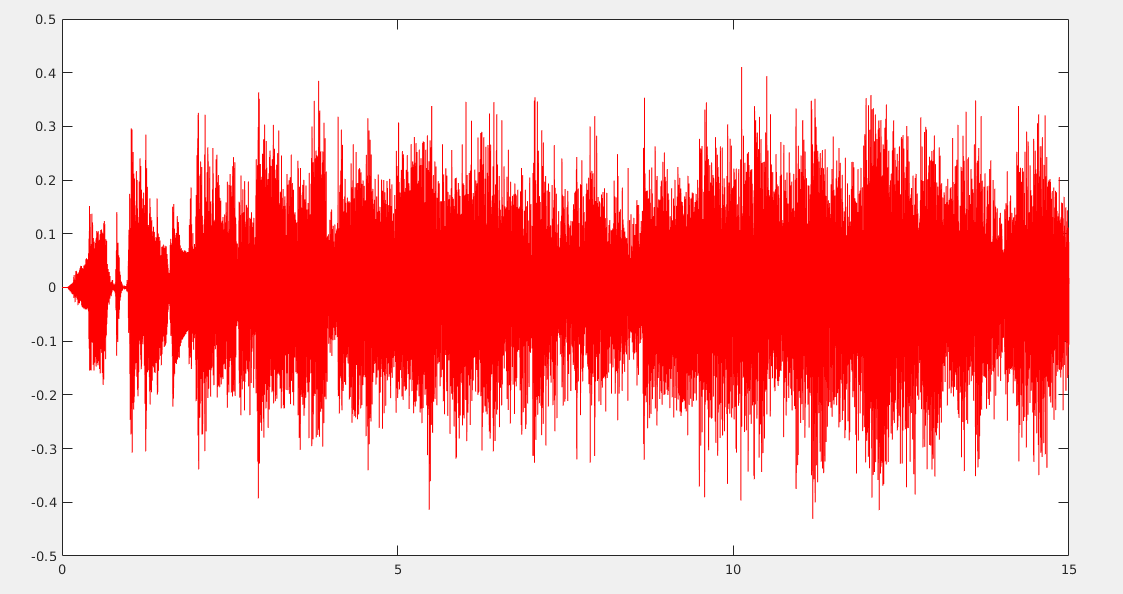
\includegraphics[width=200pt]{slike/echo_vrijeme.png}
    \centering
    \caption{Signal s dodanim odjekom u vremenu}
    \label{echo_vrijeme}
\end{figure}

Na slici \ref{komp_ulaz_spektar} prikazan je spektrogram ulaznog signala, dok je na slici \ref{echo} prikazan spektrogram
signala s dodanim odjekom. Kad se uspoređuju spektrogrami ulaznog i obrađenog signala može se zaključiti da nema
značajnih promjena u spektrogramima, što je očekivano jer dodavanjem odjeka se ne dodaju nove frekvencijske komponente.
Drugim riječima, ako je ulaznom signalu nadodan signal koji odgovara ulaznom, ali tek nakon određenog vremena u spektru
se ne očekuju nove frekvencijske komponente.


% \begin{figure}[H]
%   \centerline{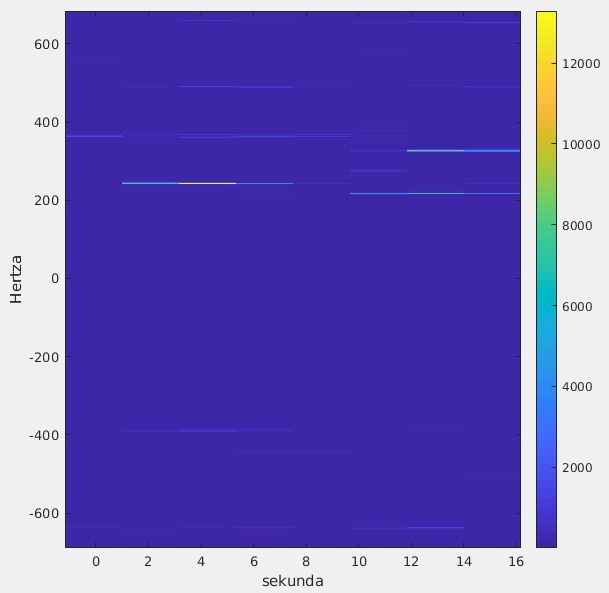
\includegraphics[height=200pt]{slike/echo_ulaz.jpeg}}
%   \caption{Spektar ualznog signala}
%   \label{echo_ulaz}
% \end{figure}

\begin{figure}[H]
  \centerline{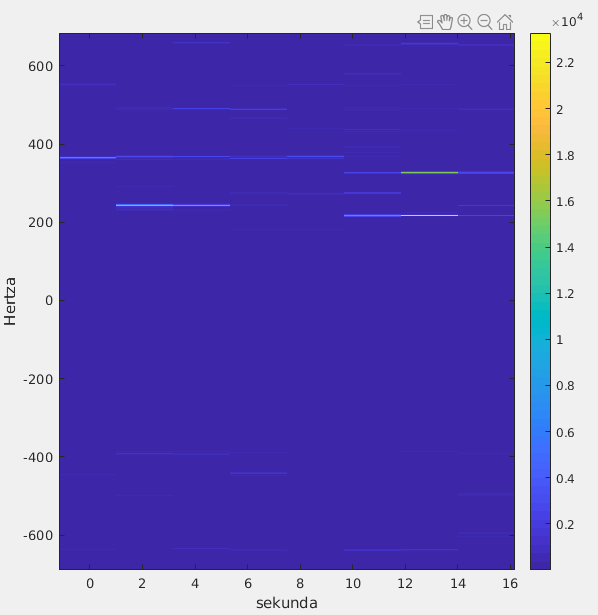
\includegraphics[height=200pt]{slike/echo.png}}
  \caption{Spektar obrađenog signala}
  \label{echo}
\end{figure}


\section{Zaključak}
Digitalna obradba signala sastavni je dio glazbene produkcije. Zvučni efekti, često nastali kao
posljedica slučajnih pogrešaka u sviranju i obradbi signala, glavni su faktori u manipulaciji zvukom.

Kompresija smanjuje dinamički raspon signala bez distorzije, bez potrebe za rezanjem
(\textit{clippingom}).

\begin{thebibliography}{00}
\bibitem{b1} Cardiff University, ``Digital Audio Effects'',
	\url{www.cs.cf.ac.uk/Dave/CM0268/PDF/10_CM0268_Audio_FX.pdf}
  \bibitem{b2} Compressor - MATLAB,
  \url{https://www.mathworks.com/help/audio/ref/compressor.html}
  \bibitem{b3} ``Dinamička obrada audiosignala'',
  \url{https://www.fer.unizg.hr/_download/repository/EAT13_Dinamicka_obrada_audio_signala_2017-18.pdf}
  \bibitem{b4} Delay-Based Effects - MATLAB,
  \url{https://www.mathworks.com/help/audio/examples/delay-based-audio-effects.html}
  \bibitem{b5} Effects Explained: Echo, Delay, and Reverb
  \url{http://www.gibson.com/News-Lifestyle/Features/en-us/effects-explained-echo-delay.aspx}
\end{thebibliography}

\end{document}
